\documentclass[10pt]{IEEEtran}
\usepackage[backend=biber,style=phys]{biblatex}
\usepackage{amsmath}
\usepackage{amsfonts}
\usepackage{amssymb}
\usepackage{caption}
\usepackage{graphicx}
\usepackage{hyperref}
\usepackage{hhline}
\usepackage{listings}
\usepackage{multirow}
\usepackage{subcaption}
\lstset{language=C++}
\usepackage{csquotes}
\usepackage{url} 
\graphicspath{{./images/}}
\addbibresource{xrayspectroscopy.bib}

\begin{document}

% Define document title and author
    \title{Energy Dispersive X-ray Spectroscopy (EDXS)}
    \author{Jamison Lahman, Brandon Coleman, and Taylor Grueser
    \thanks{Instructor: Paul King}}
    \maketitle

% Write abstract here
\begin{abstract}
Energy Dispersive X-ray Spectroscopy (EDXS) uses X-ray excitation in a sample to perform elemental analysis. Directing a charged beam of particles at a sample allows for an ejection of the sample's electrons. The ejected electron leaves a 'hole' which can then be filled by an outer shell electron, emitting an X-ray. Each element has specific X-ray energies, though some elements may overlap. Using these basic principles, we used the NORAN System Six EDXS to investigate the composition of four objects, one of which had a known composition. The known material was a U.S. Government issued dime which is theoretically composed of roughly 8\% nickel and 92\% copper. We found our dime to be approximately 35$\pm$0.75\% nickel and 65$\pm$0.75\% copper.
\end{abstract}

\section{Introduction \& Theory}
In any non-ionized atom, electrons are present outside of the nucleus. In accordance with Pauli's exclusion principle, each electron only may occupy specific positions around the nucleus and no two electrons may occupy the same position. Electrons are negatively charged and naturally repel from one-another while they are attracted to the positively charged protons in the nucleus. The balance of this attraction and repulsion gives way to shells around the nucleus which the electrons coalesce. The number of electrons, $N_e$, in a given shell $n$ is given by,
\begin{equation}
N_e = 2n^{2},
\label{eq.1}
\end{equation}
where $n$ is a positive integer. The value of $n$ is often referred to as the principle quantum number\cite{michler}. Electrons in a higher shell (one with a larger $n$ value) have a higher energy. Additionally, as the attraction of the nucleus and the electrons varies as the number of protons in the nucleus increases, so too do the transition energies.

\begin{table}[!hbt]
    \begin{center}
    \caption{Energies of X-ray Emission Lines}
    \label{tab:energies}
	\begin{tabular}{c|cccccc}
\hline 
Element & K$\alpha_1$ & K$\alpha_2$ & K$\beta_1$ & L$\alpha_1$ & L$\alpha_2$ & L$\beta_1$ \\ 
\hline 
O & 524.9 &   &  \\  
Mg & 1253.50 & 1253.60 & 1302.2 & & & \\  
Al & 1486.70 & 1486.27 & 1557.45 & & & \\  
Si & 1739.98 & 1739.38 & 1835.94 & & & \\  
Ca & 3691.68 & 3688.09 & 4012.7 & 341.3 & 341.3 & 344.9 \\ 
Mn & 5898.75 & 5887.65 & 6490.45 & 637.4 & 637.4 & 648.8 \\ 
Fe & 6403.84 & 6390.84 & 7057.98 & 705.0 & 705.0 & 718.5 \\ 
Ni & 7478.15 & 7460.89 & 8264.66 & 851.5 & 851.5 & 868.8 \\ 
Cu & 8047.78 & 8027.83 & 8905.29 & 929.7 & 929.7 & 949.8 \\ 
Zn & 8638.86 & 8615.78 & 9572.0 & 1011.7 & 1011.7 & 1034.7 \\ 
\hline
	\end{tabular}
	\medskip \\
    Various emission energies (in eV) from common elements\cite{xdb}. Transition paths are those found in Fig. \ref{fig:paths}.
	\end{center}
\end{table}

If an electron in a lower shell is removed, an electron from a higher shell may transition to fill the lower shell. Since a lower shell corresponds to a lower energy, the transitioning electron emits radiation in the process. Using a charged beam of particles, either electrons, protons or x-rays, the inner electrons around an atom can be ejected. The resulting electron 'hole' can be filled by an outer electron, thus potentially emitting an X-ray. The light emitted is roughly equal the energy differences of the two shells and values vary between elements.

\begin{figure}[t]
       \begin{center}
       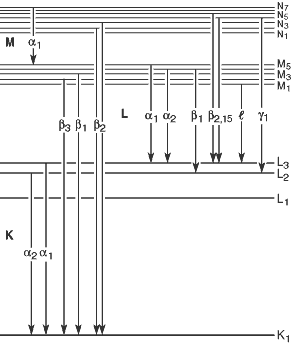
\includegraphics[width=\columnwidth]{Sec1201.png}
       \caption{Transition paths which produce the various X-ray emissions.\cite{xdb}}
       \label{fig:paths}
       \end{center}
\end{figure}

\section{Experimental Details}
The apparatus for this experiment was the we used the NORAN System Six EDXS. The EDXS software was created in Labview and performs data acquisition and rudimentary analysis via the XIA Saturn pulse processor. The duration of each sample was 100 seconds run time though the real time varied somewhat. We had four objects, one of which had a known composition. The known material was a U.S. Government issued dime which is theoretically composed of roughly 8\% nickel and 92\% copper\cite{mint}. The remaining three objects were a broken cap, a metal, and a rock. Each had an unknown composition and cannot be compared to literature.

\begin{center}
\begin{figure*}[!t]
    \begin{subfigure}[!t]{0.25\textwidth}
        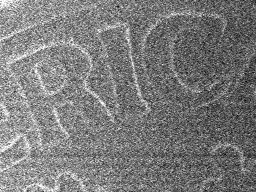
\includegraphics[width=\textwidth]{Dime_1}
        \caption{Object 1, location 1.}
        \label{fig:Dime_1}
    \end{subfigure}\quad
    ~ %add desired spacing between images, e. g. ~, \quad, \qquad, \hfill etc. 
      %(or a blank line to force the subfigure onto a new line)
    \begin{subfigure}[!t]{0.25\textwidth}
        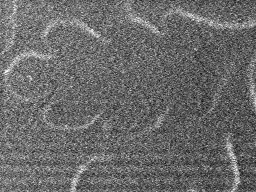
\includegraphics[width=\textwidth]{Dime_2}
        \caption{Object 1, location 2.}
        \label{fig:Dime_2}
    \end{subfigure}\hfill
    ~ %add desired spacing between images, e. g. ~, \quad, \qquad, \hfill etc. 
    %(or a blank line to force the subfigure onto a new line)
    \begin{subfigure}[!t]{0.41\textwidth}
        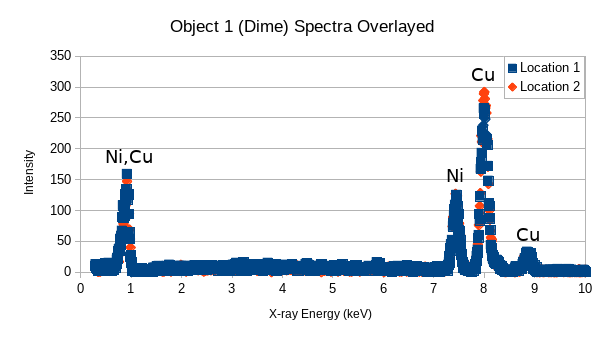
\includegraphics[width=\textwidth]{Object1}
        \label{fig:Object1}
    \end{subfigure}
    \caption{The optical images of the two locations and the corresponding spectrum of the United States Government dime. The prominent peaks are labeled indicating the elements in the sample.}
    \label{fig:objects1}
\end{figure*}

\begin{figure*}[!hbtt]
    \begin{subfigure}[!hbt]{0.25\textwidth}
        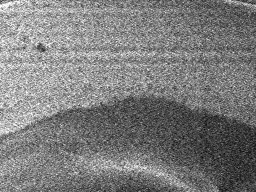
\includegraphics[width=\textwidth]{Object2_1}
        \caption{Object 2, location 1.}
        \label{fig:Object2_1}
    \end{subfigure}\quad
    ~ %add desired spacing between images, e. g. ~, \quad, \qquad, \hfill etc. 
      %(or a blank line to force the subfigure onto a new line)
    \begin{subfigure}[!hbt]{0.25\textwidth}
        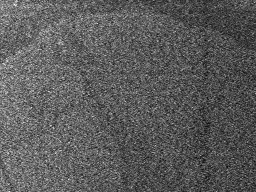
\includegraphics[width=\textwidth]{Object2_2}
        \caption{Object 2, location 2.}
        \label{fig:Object2_2}
    \end{subfigure}\hfill
    ~ %add desired spacing between images, e. g. ~, \quad, \qquad, \hfill etc. 
    %(or a blank line to force the subfigure onto a new line)
    \begin{subfigure}[!hbt]{0.41\textwidth}
        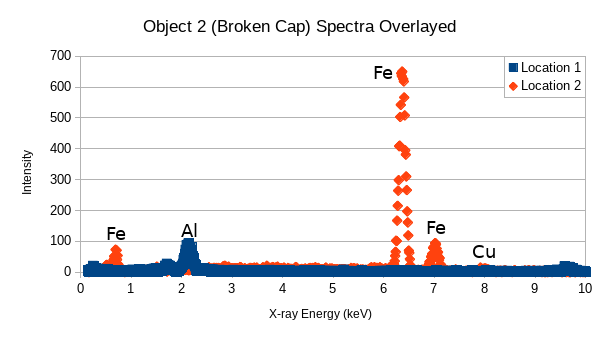
\includegraphics[width=\textwidth]{Object2}
        \label{fig:Object2}
    \end{subfigure}
    \caption{The optical images of the two locations and the corresponding spectrum of the broken cap. The prominent peaks are labeled indicating the elements in the sample.}
    \label{fig:objects2}
\end{figure*}

\begin{figure*}[!hbt]
    \begin{subfigure}[!hbt]{0.25\textwidth}
        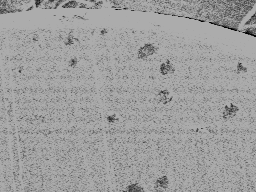
\includegraphics[width=\textwidth]{Object3_1}
        \caption{Object 3, location 1.}
        \label{fig:Object3_1}
    \end{subfigure}\quad
    ~ %add desired spacing between images, e. g. ~, \quad, \qquad, \hfill etc. 
      %(or a blank line to force the subfigure onto a new line)
    \begin{subfigure}[!hbt]{0.25\textwidth}
        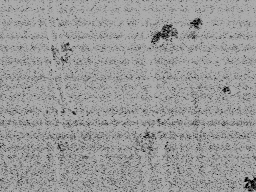
\includegraphics[width=\textwidth]{Object3_2}
        \caption{Object 3, location 2.}
        \label{fig:Object3_2}
    \end{subfigure}\hfill
    ~ %add desired spacing between images, e. g. ~, \quad, \qquad, \hfill etc. 
    %(or a blank line to force the subfigure onto a new line)
    \begin{subfigure}[!hbt]{0.41\textwidth}
        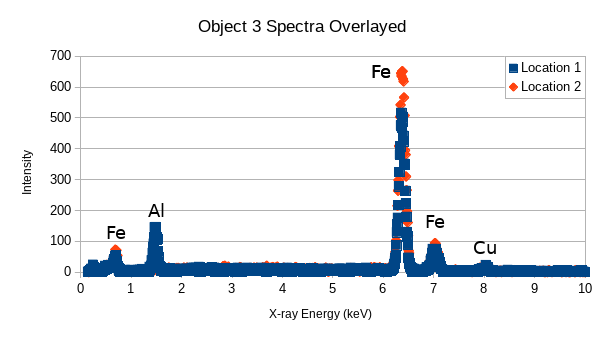
\includegraphics[width=\textwidth]{Object3}
        \label{fig:Object3}
    \end{subfigure}
    \caption{The optical images of the two locations and the corresponding spectrum of the broken cap. The prominent peaks are labeled indicating the elements in the sample.}
    \label{fig:objects3}
\end{figure*}

\begin{figure*}[!hbt]
    \begin{subfigure}[!hbt]{0.19\textwidth}
        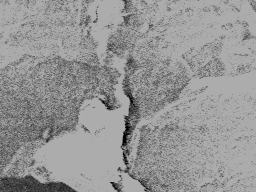
\includegraphics[width=\textwidth]{Object4_1}
        \caption{Object 4, location 1.}
        \label{fig:Object4_1}
    \end{subfigure}
    ~ %add desired spacing between images, e. g. ~, \quad, \qquad, \hfill etc. 
      %(or a blank line to force the subfigure onto a new line)
    \begin{subfigure}[!hbt]{0.19\textwidth}
        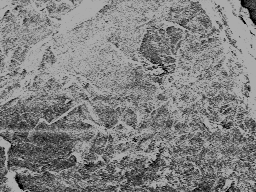
\includegraphics[width=\textwidth]{Object4_2}
        \caption{Object 4, location 2.}
        \label{fig:Object4_2}
    \end{subfigure}    
    ~ %add desired spacing between images, e. g. ~, \quad, \qquad, \hfill etc. 
      %(or a blank line to force the subfigure onto a new line)
    \begin{subfigure}[!hbt]{0.19\textwidth}
        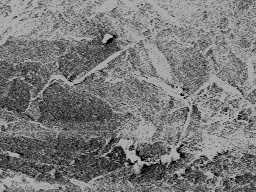
\includegraphics[width=\textwidth]{Object4_3}
        \caption{Object 4, location 3.}
        \label{fig:Object4_3}
    \end{subfigure}\hfill
    ~ %add desired spacing between images, e. g. ~, \quad, \qquad, \hfill etc. 
    %(or a blank line to force the subfigure onto a new line)
    \begin{subfigure}[!hbt]{0.40\textwidth}
        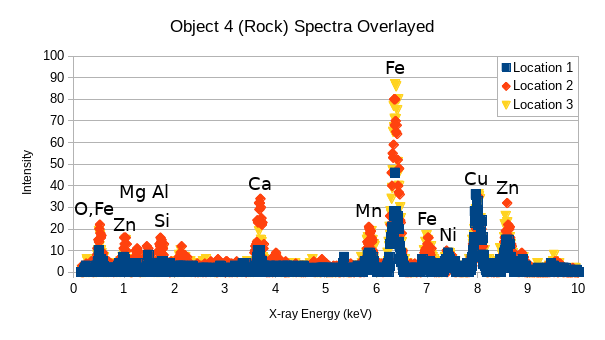
\includegraphics[width=\textwidth]{Object4}
        \label{fig:Object4}
    \end{subfigure}
    \caption{The optical images of the two locations and the corresponding spectrum of the unknown rock. The prominent peaks are labeled indicating the elements in the sample.}
    \label{fig:objects4}
\end{figure*}
\end{center}

\section{Data}
    
        \begin{table}[!hpbt]
      \begin{center}
        \normalsize{Relative Composition of the Dime}
        \begin{tabular}{|c|c|c|c|c|}	
		   \hline        	
		   Element & Location & Atom \% & Error \\
            \hline
            \multirow{2}{*}{Ni} & 1 & 26.18 & 0.53 \\
            \hhline{~----}
	        & 2 & 25.90 & 0.51 \\
	        \hline
            \multirow{2}{*}{Cu} & 1 & 73.81 & 0.53 \\
            \hhline{~----}
            & 2 & 74.10 & 0.51 \\
            \hline
       \end{tabular}
       \caption{The relative abundances of nickel and copper at two points on the dime.}
       \label{tab:dime}
      \end{center}
    \end{table}
    
        \begin{table}[!hpbt]
      \begin{center}
        \normalsize{Relative Composition of the Broken Cap}
        \begin{tabular}{|c|c|c|c|c|}	
		   \hline        	
		   Element & Location & Atom \% & Error \\
            \hline
            \multirow{2}{*}{Si} & 1 & 22.98 & 3.15 \\
            \hhline{~----}
	        & 2 & 100 & 0.42 \\
	        \hline
            \multirow{2}{*}{Ca} & 1 & 5.23 & 2.33 \\
            \hhline{~----}
            & 2 & 0 & 0 \\
            \hline           
            \multirow{2}{*}{Br} & 1 & 5.83 & 9.06 \\
            \hhline{~----}
            & 2 & 0 & 0 \\
            \hline           
             \multirow{2}{*}{Au} & 1 & 65.96 & 12.03 \\
            \hhline{~----}
            & 2 & 0 & 0 \\
            \hline
       \end{tabular}
       \caption{The relative abundances of silicon, calcium, bromine and gold at two points on the broken cap.}
       \label{tab:object2}
      \end{center}
    \end{table}
    
            \begin{table}[!hpbt]
      \begin{center}
        \normalsize{Relative Composition of the Metal}
        \begin{tabular}{|c|c|c|c|c|}	
		   \hline        	
		   Element & Location & Atom \% & Error \\
            \hline
            \multirow{2}{*}{Fe} & 1 & 78.58 & 1.08 \\
            \hhline{~----}
	        & 2 & 97.93 & 1.42 \\
	        \hline
            \multirow{2}{*}{Al} & 1 & 18.88 & 0.45 \\
            \hhline{~----}
            & 2 & 0.16 & 0.33 \\
            \hline           
            \multirow{2}{*}{Cu} & 1 & 2.54 & 0.36 \\
            \hhline{~----}
            & 2 & 2.07 & 0.98 \\
            \hline           
       \end{tabular}
       \caption{The relative abundances of iron, aluminium and copper at two points on the metal object.}
       \label{tab:object3}
      \end{center}
    \end{table}
    
\begin{figure}[!h]
       \begin{center}
       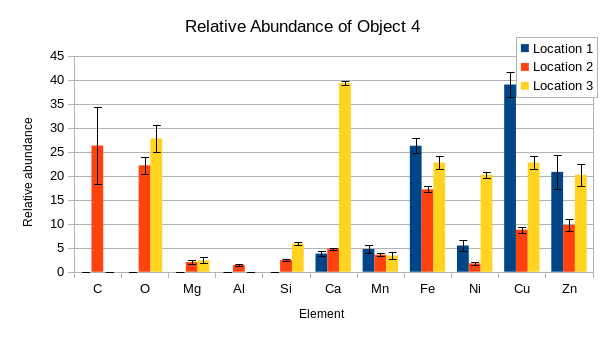
\includegraphics[width=\columnwidth]{Object4Analysis}
       \caption{The relative abundances of all detected elements in the mineral sample. Some elements, such as carbon, are found sporadically and have a large error. Because of the method the EDXS software, it is likely these are false positives.}
       \label{fig:all}
       \end{center}
\end{figure}
           
\begin{table}[!hpbt]
      \begin{center}
        \normalsize{Mutual, Relative Composition of the Mineral}
        \begin{tabular}{|c|c|c|c|c|}	
		   \hline        	
		   Element & Location & Atom \% & Error \\
            \hline
            \multirow{3}{*}{Ca} & 1 & 3.78 & 0.51 \\
            \hhline{~----}
	        & 2 & 10.48 & 0.55 \\
	        \hhline{~----}
	        & 3 & 4.06 & 3.89 \\
	        \hline
            \multirow{3}{*}{Mn} & 1 & 4.73 & 0.77 \\
            \hhline{~----}
            & 2 & 7.75 & 0.72 \\
            \hhline{~----}
	        & 3 & 6.11 & 0.70 \\	      
	        \hline  
            \multirow{3}{*}{Fe} & 1 & 26.24 & 1.55 \\
            \hhline{~----}
            & 2 & 37.55 & 1.42 \\
            \hhline{~----}
            & 3 & 41.25 & 1.43 \\
            \hline
            \multirow{3}{*}{Ni} & 1 & 5.47 & 1.15 \\
            \hhline{~----}
            & 2 & 3.79 & 0.68 \\
            \hhline{~----}
            & 3 & 3.53 & 0.71 \\
            \hline
            \multirow{3}{*}{Cu} & 1 & 38.98 & 2.58 \\
            \hhline{~----}
            & 2 & 19.17 & 1.40 \\
            \hhline{~----}
            & 3 & 23.86 & 1.50 \\
            \hline
            \multirow{3}{*}{Zn} & 1 & 20.80 & 3.59 \\
            \hhline{~----}
            & 2 & 21.27 & 2.56 \\
            \hhline{~----}
            & 3 & 21.18 & 2.45 \\
            \hline
       \end{tabular}
       \caption{The relative abundances elements that were found at each location. Elements found at only one spot, such as carbon, were omitted.}
       \label{tab:object4}
      \end{center}
    \end{table}    
    
\begin{figure}
       \begin{center}
       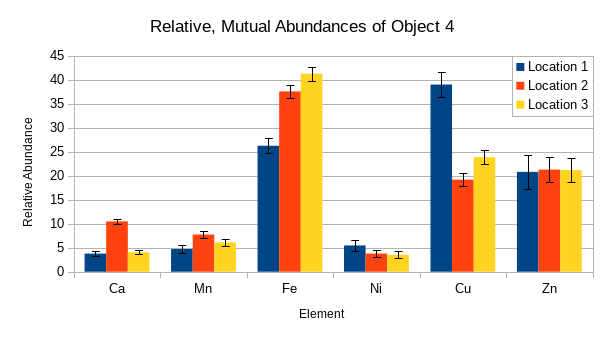
\includegraphics[width=\columnwidth]{Object4Mutual}
       \caption{After eliminating the sporadic elements, we find that the relative abundances to be rather uniform across the mineral. At location 1, there appears to be an excess of iron in place of copper while location 2 has an excess of calcium.}
       \label{fig:mutual}
       \end{center}
\end{figure}
    
\section{Results}

Nickel and copper are relatively close on the periodic table, so their mass contributions are going to be roughly equal to their atom contribution. Nevertheless, the amount of nickel in our dime greatly disagrees with the literature value supplied by the U.S. Government. Regardless, we found within one standard error a homogeneous composition of the Dime. From Fig. \ref{fig:objects2}, it is easy to see the composition of the cap is not uniform.

In one location of the metal, aluminium appears to make about a 19\% contribution to the number of atoms while it is barely present in the second location. Focusing only on the iron to copper ratio by integrating their specific peaks, we find that the Cu/Fe ratio at the two locations are,
\[
\frac{\text{Cu}}{\text{Fe}}_1 = 2.63\text{E-2} \pm 1.28\text{E-3}
\]
\[
\frac{\text{Cu}}{\text{Fe}}_2 = 2.11\text{E-2} \pm 1.02\text{E-3}
\]
Performing error propagation, we find that roughly 22\% of the error comes from the copper. In total, it is reasonable to conclude that the copper to iron ratio is changing throughout the metal.

As for the mineral. some elements, such as carbon, are detected sporadically and had a large error. Because of the method the EDXS software, it is likely these were wrongly attributed. After eliminating the sporadic elements, we find that the relative abundances to be rather uniform across the mineral. At location 1, there appears to be an excess of iron in place of copper while location 2 has an excess of calcium.
\section{Conclusion}

Despite only having one object with a known composition, the elements detected in the other objects agrees with our intuition. We found our U.S. Government issued dime to be approximately 35$\pm$0.75\% nickel and 65$\pm$0.75\% copper while it is theoretically composed of roughly 8\% nickel and 92\% copper. It is likely that there is a defect in the composition evaluation of the software as opposed to an unusual composition of our dime. In contrast, It would make sense that something plastic like a cap would be dominated by silicon. Likewise, iron, copper, and aluminium are all commonly associated with the metals and the rock was composed of many, various elements. Despite there being some slight deviation across the mineral, there were constant contributions by elements such as zinc and nickel.

\section{acknowledgments}
I would like to thank my lab partners, Brandon Coleman and Taylor Grueser, who helped with the setup, data acquisition and analysis for this report.
\printbibliography

\end{document}

% This is how you include a eps figure in your document. LaTeX only accepts EPS or TIFF files.
%    \begin{figure}[!hbt]
        % Center the figure.
%        \begin{center}
        % Include the eps file, scale it such that it's width equals the column width. You can also put width=8cm for example...
%        \includegraphics[width=\columnwidth]{}
        % Create a subtitle for the figure.
%       \caption{Simulation results on the AWGN channel. Average throughput $k/n$ vs $E_s/N_0$.}
        % Define the label of the figure. It's good to use 'fig:title', so you know that the label belongs to a figure.
%        \label{fig:tf_plot}
%        \end{center}
%    \end{figure}

    % This is how you define a table: the [!hbt] means that LaTeX is forced (by the !) to place the table exactly here (by h), or if that doesnt work because of a pagebreak or so, it tries to place the table to the bottom of the page (by b) or the top (by t).
%    \begin{table}[!hbt]
        % Center the table
%        \begin{center}
        % Title of the table
%        \caption{Simulation Parameters}
%        \label{tab:simParameters}
        % Table itself: here we have two columns which are centered and have lines to the left, right and in the middle: |c|c|
%        \begin{tabular}{|c|c|}
            % To create a horizontal line, type \hline
%            \hline
            % To end a column type &
            % For a linebreak type \\
%            Information message length & $k=16000$ bit \\
%            \hline
%            Radio segment size & $b=160$ bit \\
%            \hline
%            Rate of component codes & $R_{cc}=1/3$\\
%            \hline
%            Polynomial of component encoders & $[1 , 33/37 , 25/37]_8$\\
%            \hline
%        \end{tabular}
%        \end{center}
%    \end{table}

% You can cite a book or paper by using \cite{reference}.

% You can reference tables and figure by using the \ref{label} command. Each table and figure needs to have a UNIQUE label.
%Figures and tables should be labeled and numbered, such as in Table~\ref{tab:simParameters} and Fig.~\ref{fig:tf_plot}.
